\documentclass[tikz,multi,border=10pt]{standalone}
    \usepackage{color}
    \usetikzlibrary{shadows,arrows.meta,positioning,backgrounds,fit}
    
    % Define block styles
    \tikzset{%
      materia/.style={draw, fill=blue!20, text width=6.0em, text centered, minimum height=1.5em,drop shadow},
      etape/.style={materia, text width=8em, minimum width=10em, minimum height=3em, rounded corners, drop shadow},
      texto/.style={above, text width=6em, text centered},
      linepart/.style={draw, thick, color=black!50, -LaTeX, dashed},
      line/.style={draw, thick, color=black!50, -LaTeX},
      ur/.style={draw, text centered, minimum height=0.01em},
      back group/.style={fill=yellow!20,rounded corners, draw=black!50, dashed, inner xsep=15pt, inner ysep=10pt},
    }
    
    \newcommand{\etape}[2]{node (p#1) [etape] {#2}}
    
    \newcommand{\transreceptor}[3]{%
      \path [linepart] (#2) -- (#1.east);}
    
    \begin{document}
    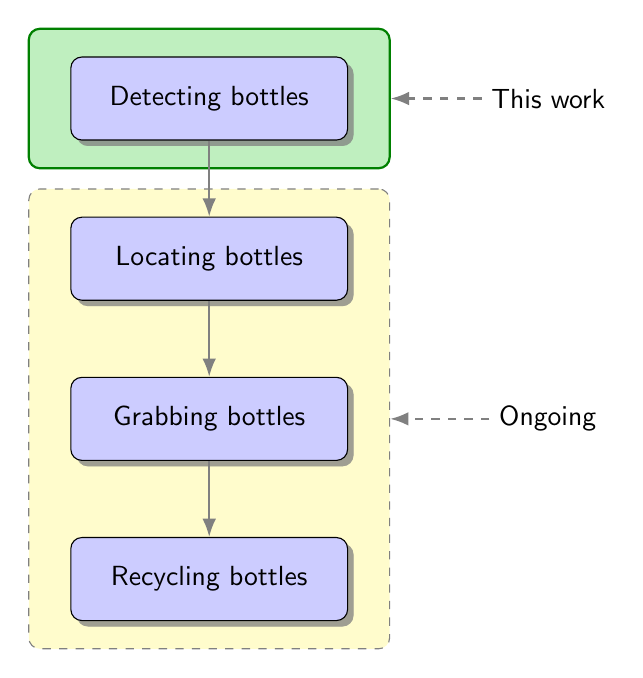
\begin{tikzpicture}[font=\sffamily]
    
      % Draw diagram elements
      \path \etape{1}{Detecting bottles};
    
      \path (p1.south)+(0.0,-1.5) \etape{2}{Locating bottles};
      \path (p2.south)+(0.0,-1.5) \etape{3}{Grabbing bottles};
      \path (p3.south)+(0.0,-1.5) \etape{4}{Recycling bottles};
 
      % Draw arrows between elements
      \path [line] (p1.south) -- node [above] {} (p2);
      \path [line] (p2.south) -- node [above] {} (p3);
      \path [line] (p3.south) -- node [above] {} (p4);
    
      \begin{scope}[on background layer]
        \node (bk1) [draw, thick, green!50!black, fill=green!75!black!25, rounded corners, fit=(p1), inner xsep=15pt, inner ysep=10pt] {};
        \node (bk2) [back group] [fit=(p2) (p3) (p4)] {};
      \end{scope}
    
      \path (bk1.east)+(+2.0,0) node (ur1) {This work};
      \path (bk2.east)+(+2.0,0) node (ur2) {Ongoing};

      \transreceptor{bk1}{ur1};
      \transreceptor{bk2}{ur2};

    \end{tikzpicture}
    \end{document}